\chapter{Generation of the road structure}
\label{app:appendix_a}

\graphicspath{{appendix_a/figures/}} % path to the figures folder of this chapter
 \begin{figure}
\centering
    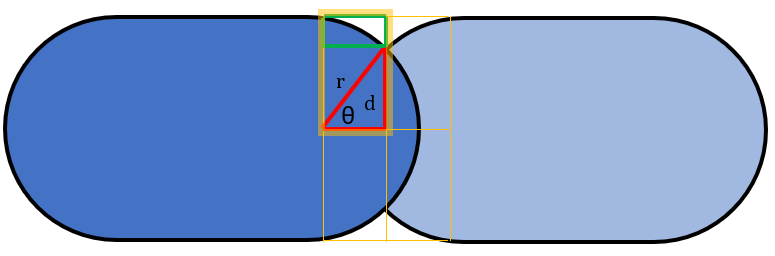
\includegraphics[width=0.8\textwidth]{appendix_a/figures/calsurface.PNG}
   \caption{An overlap of two stadium shapes can be determined by using trigonometry to calculate the surface of the different sectors}
   \end{figure}
  
\begin{figure}
\centering
  \begin{subfigure}[b]{0.6\textwidth}
    \includegraphics[width=\textwidth]{appendix_a/figures/Step1.PNG}
    \caption{Filament is extruded out of the nozzle and expans due to dye swelling}
  \end{subfigure}
  %
  \begin{subfigure}[b]{0.6\textwidth}
    \includegraphics[width=\textwidth]{appendix_a/figures/Step2.PNG}
    \caption{By applying a horizontal contraint (the buildplate) an ellipse is generated}
  \end{subfigure}
  \\
    \begin{subfigure}[b]{0.6\textwidth}
    \includegraphics[width=\textwidth]{appendix_a/figures/Step3.PNG}
    \caption{When the nozzle is place at the layer height, the road is compressed and expands towards a stadium shape}
  \end{subfigure}
  %
  \begin{subfigure}[b]{0.6\textwidth}
    \includegraphics[width=\textwidth]{appendix_a/figures/Step4.PNG}
    \caption{The stadium shapes are placed with an overlap to fill in the porosity and create a larger contact surface}
  \end{subfigure}
  \\
  \caption{The generation of the mesostructure results from the extrusion process, which is explained in these subfigures}
  \end{figure}
  
 
  
%Nowadays, a smart use of the appendix is becoming more and more important. People do not have enough time to read long documents anymore (that's the truth...). So, the best journal articles (Nature \& Science) adopted a format where there is a short ``main body'' and then there is a long ``Supporting Information'' (which is the Appendix of a thesis).

%My general advice is for you to do the same. Write concisely the essential information that you put in the main body. Focus on the main message and the key storyline. Then, leave to the appendices all supporting results, modeling details, secondary arguments, etc.